\documentclass{article}
\usepackage[T1]{fontenc}
\usepackage{lmodern}
\usepackage{graphicx}
\usepackage{amsmath,amssymb}
\usepackage[a4paper,margin=2cm]{geometry}
\usepackage[absolute,overlay]{textpos}
\setlength{\TPHorizModule}{1mm}
\setlength{\TPVertModule}{1mm}
\usepackage[indonesian]{babel}
\usepackage{hyperref}
\setlength{\emergencystretch}{2em}
% unit: Halaman 64

\begin{document}

% === Halaman 64 (llm) ===

\section*{How to Hack a Computer Using Just An Image}
\noindent Monday, June 01, 2015 $\bullet$ Swati Khandelwal

\vspace{20mm}

Next time when someone sends you a photo of a cute cat or a hot chick then be careful before you CLICK on the image to view --- it might hack your machine.

Yes, the normal looking images could hack your computers --- thanks to a technique discovered by security researcher \textit{Saumil Shah} from India.

\vspace{59.40mm}

Dubbed \quot{Stegospolit\quot, the technique lets hackers hide malicious code inside the pixels of an image, hiding a malware exploit in plain sight to infect target victims.

\textbf{Just look at the image and you are HACKED!}

\url{http://thehackernews.com/2015/06/Stegospolit-malware.html}

% deskripsi: Screenshot artikel yang menunjukkan gambar kucing dengan teks 'THIS PICTURE CAN HACK YOUR COMPUTER' dan latar belakang kode biner.
% bbox normalisasi: [0.1700, 0.1300, 0.6600, 0.5900]
\begin{textblock*}{102.90mm}(35.70mm,38.61mm)
\noindent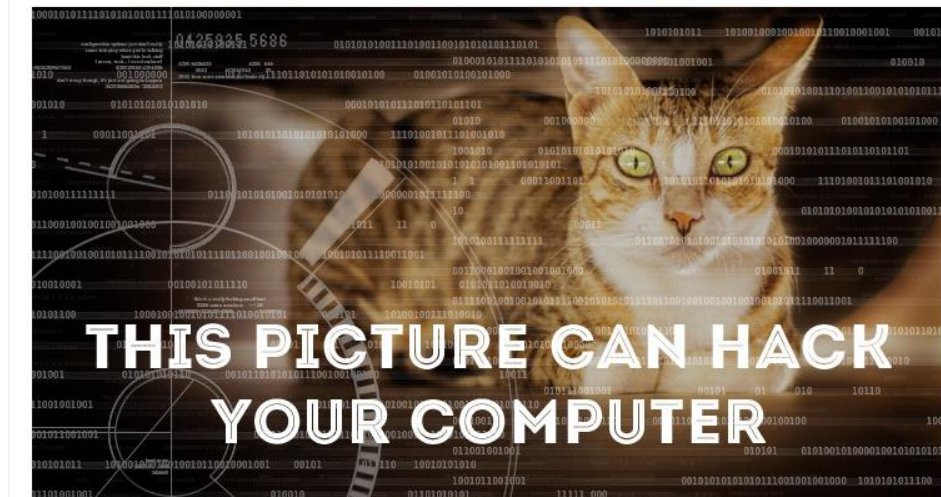
\includegraphics[width=102.90mm,height=136.62mm]{../../images/llm/page_064_img_01.png}%
\end{textblock*}

% deskripsi: Screenshot layar terminal komputer berwarna hitam dengan teks hijau bertuliskan 'ACCESS GRANTED'.
% bbox normalisasi: [0.7100, 0.6400, 0.8800, 0.8400]
\begin{textblock*}{35.70mm}(149.10mm,190.08mm)
\noindent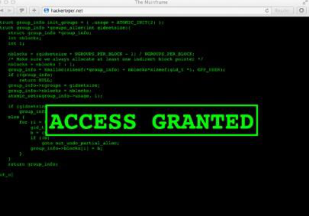
\includegraphics[width=35.70mm,height=59.40mm]{../../images/llm/page_064_img_02.png}%
\end{textblock*}

\end{document}
